
% ------------------------------------------------------------------
% Einstellen der Grundzüge des Layouts, z. B. Blattgröße
%------------------------------------------------------------------
\documentclass[a4paper,twoside=false,fontsize=6,numbers=noenddot,DIV=16]{scrreprt}
\usepackage[landscape, left=5mm, right=5mm, top=5mm, bottom=5mm]{geometry}
\pagestyle{empty}

%------------------------------------------------------------------
% Importieren den notwendigen packages
%------------------------------------------------------------------
% math stuff
\usepackage[nosumlimits, nointlimits, fleqn]{amsmath}
\usepackage{amssymb}

% Bildumgebungen
\usepackage{graphicx}
\usepackage{float}
\usepackage[dvipsnames]{xcolor}	

% Tabellenumgebung
\usepackage{longtable}				% Tabellen mit Seitenumbruch
\renewcommand\arraystretch{1.4}   		% Tabellen: Zeilen um Faktor x vergrößern
\usepackage{booktabs}				% professionelle Tabellen (Grundeinstellung bei Excel2LaTeX Excel-PlugIn)

% Sonstige Umgegebungen
\usepackage{listings}	
\usepackage[ngerman]{babel}
% \usepackage[latin1]{inputenc}
\usepackage[T1]{fontenc}

% Drei Spalten nebeneinander
\usepackage{multicol}

% Colorboxen
\usepackage{tcolorbox}

% Package um Aufzählungen zu "verschönern"
\usepackage{enumitem}

% Todos hervorheben
\usepackage[obeyDraft]{todonotes}

% Um Einheiten richtig darzustellen 
\usepackage[per-mode=symbol]{siunitx}

% Für eine Verlinkung im Inhaltsverzeichnis.
% Dieses Paket möglichst als letztes einbinden falls Fehler auftreten!!!
\usepackage{hyperref}
\hypersetup{
    %bookmarks=true,
    unicode=false,
    pdfborder={0 0 0},
    pdftoolbar=true,
    pdfmenubar=true,
    pdffitwindow=false,
    pdfstartview={FitH},
    pdftitle={HelpSheet},
    pdfnewwindow=true,
    colorlinks=false,
    linkcolor=red,
    citecolor=green,
    filecolor=magenta,
    urlcolor=cyan
}

\usepackage{blindtext}
\usepackage{empheq}

%%% Local Variables:
%%% mode: latex
%%% TeX-master: "../HelpSheet"
%%% End:


%------------------------------------------------------------------
% Weitere Einstellungen (Farben / Numerierungstiefen)
%------------------------------------------------------------------
\include{tex/settings}

% New definitions
\newcommand{\argmin}{\arg\!\min}
\newcommand{\argmax}{\arg\!\max}
\newcommand{\diff}{\mathrm{d}}
\newcommand{\cov}{\mathrm{cov}}
\newcommand{\var}{\mathrm{var}}
\newcommand{\matrixroot}[1]{#1^{\frac{1}{2}}}
\newcommand{\ti}[2]{#1_\mathrm{#2}}
\newcommand{\inv}{^{-1}}
\newcommand{\trans}{^\top}
\newcommand{\norm}[1]{\lVert#1\rVert}

%------------------------------------------------------------------
% Dokumentbeginn
%------------------------------------------------------------------
\begin{document}

\setlength{\columnsep}{0.4cm}
\setlength{\columnseprule}{0pt}
\begin{multicols*}{3}
	\begin{tcolorbox}[colback=blue!5!white,colframe=blue!75!black,title=\textbf{Basics}]

\textbf{ \textsc{Newton} Root-finding problem}\\
for $R:\mathbb{R}^n\rightarrow \mathbb{R}^n$ find $z$ such that $R(z) = 0$

Root-finding series:
\begin{flalign*}
z_{k+1}=z_k - (\nabla_z R(z_k))^{-1}\cdot R(z_k) \quad \text{, with }\nabla_x f(x) := \left( \frac{\partial f(x)}{\partial x} \right)^\top
\end{flalign*}
General {\textsc Newton} type method (NT-method):
\begin{flalign*}
z_{k+1}=z_k - M_k^{-1}\cdot R(z_k)\ |\ M_k\approx \nabla_z R(z_k) \text{(invertible apporximation)}
\end{flalign*}\\

\textbf{ Local-contraction theorem} for \textsc{Newton} type iterations:
\begin{flalign*}
  \norm{z_{k+1}-z^*}\le
  \left(
    \kappa_k+\frac{\omega}{2}\norm{z_k-z^*}
  \right)\norm{z_k-z^*}\end{flalign*}
  \begin{flalign*}
  \mathrm{if}\ \exists \omega < \infty, \kappa <1\ \mathrm{such\ that}\\
  \norm{M_k^{-1}(\nabla_z R(z_k)-\nabla_z R(z)} \le \omega \norm{z_k -z}\ 
  (\textsc{Lipschitz}\mathrm{-condition})\\
  \norm{M_k^{-1}(\nabla_z R(z_k) - M_k)} \le  \kappa_k \le \kappa\
  (\mathrm{compatibility\ condition})\\
  \mathrm{and}\ \norm{z_0-z^*}<\frac{2(1-\kappa)}{\omega}
\end{flalign*}
Notes:
\begin{itemize}
\item $R(z^*)=0$
\item $\kappa=0$ for exact \textsc{Newton} $\to$ quadratic convergence
\item $\kappa_k \to 0$ for quasi \textsc{Newton} $\to$ super-linear convergence
\item $\kappa < 1$ for \textsc{Gauss-Newton} $\to$ linear convergence\\
\end{itemize}

\textbf{Tight condition for local convergence}
\begin{flalign*}
	\ti{\kappa}{exact}=\rho \left(M(z^*)\inv \left(M(z^*) - \nabla_z R(z^*)\right)\right)
	\left\{
	\begin{array}{cl}
		< 1: &\mathrm{converges\ to\ }z^* \\
		> 1: &\mathrm{diverges}
	\end{array}
	\right.
\end{flalign*}
\begin{itemize}
	\item Argument in $\rho$: Difference of approximate of Jacobian at $z^*$
	\item \textit{``spectral radius''} $\rho(A):=\max (|\lambda|\in \mathrm{eig}(A))$\\
\end{itemize} 
\tcblower
\textbf{\textsc{Lipschitz}-condition}
\begin{flalign*}
	\norm{f(x) - f(y)} \leq L \cdot \norm{x - y} \quad \text{for $L \leq \infty$ }
\end{flalign*}
$\Rightarrow$ an IVP has a unique solution if for the dynamics $f$ the above holds\\

\textbf{Convexity} if $\forall x,y \in \Omega, t \in [0,1]:$
\begin{flalign*}
	x + t (y-x) \in \Omega &\to \Omega \text{ is convex set} \\
	f(x+t(y-x)) \leq t (f(x) - f(y)) &\to f \text{ is convex function}
\end{flalign*}
The feasible set $\Omega$ is convex if $g$ is affine and $h_i \leq 0$ are convex.\\

\textbf{Globalization} to reach region of local convergence\\

\textbf{\textsc{Armijo}-condition}\\
For a given merrit function $V(z) = \frac{1}{2} \norm{R(z)}^2_2$ and the exact newton-step $p(z) = - J(z)^{-1} R(z)$,  exists  $\alpha \in (0,1]$, such that
\begin{flalign*}
	V(z+\alpha p(z)) \leq V(z) + \alpha \gamma \nabla V(z)^\top p(z) \quad \gamma \in (0, \frac{1}{2})
\end{flalign*}
decrease step length $\alpha$ if AC is not fulfilled: $\alpha = \beta \alpha$, \; $\beta \in (0,1]$.\\

% \textbf{MPC} - Realtime-Strategies:

% Offline Precomputation
% \begin{itemize}
% 	\item Compute Feedback Laws $u^N_{MPC} (\cdot)$ "curse of dimensionality"
% 	\item Factorize matrices
% 	\item Code generation (code optimization)
% 	\item Model simplification
% \end{itemize}

% Preparation and Feedback Phase\\
% $x_k$ delay \hspace{.5mm} $u_k$ \hspace{.5cm}prepare \hspace{1.cm} $x_{k+1}$ delay $u_{k+1}$ \hspace{.2cm}prepare\\
% {\textcolor{black}{\rule{1mm}{2mm}}}{\textcolor{red}{\rule{1.2cm}{1mm}}}{\textcolor{blue}{\rule{1mm}{2mm}}}{\textcolor{green}{\rule{3cm}{1mm}}}{\textcolor{black}{\rule{1mm}{2mm}}}{\textcolor{red}{\rule{1.2cm}{1mm}}}{\textcolor{blue}{\rule{1mm}{2mm}}}{\textcolor{green}{\rule{1.5cm}{1mm}}}\\
% Delay Compenasation by Prediction\\
% Online Techniques
% \begin{itemize}
% 	\item Iterate while problem changes
% 	\item Parallelization
% 	\item Adapt to CPU
% \end{itemize}

% Warmstart and Shifting Methods
% \begin{itemize}
% 	\item Warmstart without shifting
% 	\item shift, copy last state, or use clever alternative
% \end{itemize}

\end{tcolorbox}


%%% Local Variables:
%%% mode: latex
%%% TeX-master: "../HelpSheet"
%%% End:
	\begin{tcolorbox}[colback=green!5!white,colframe=green!75!black,title=\textbf{Karush-Kuhn-Tucker
    (KKT) Conditions}]
	\textbf{Problem:\hspace{1.7cm} Linear: \hspace{1.3cm} Linear-Quadratic:}\\
\begin{minipage}{0.33\columnwidth}
	\begin{empheq}[box=\fbox]{align*}
		\min_w &\ f(w) \\
		\mathrm{s.t.} &\ g(w)=0 \\
		&\ h(w) \le 0
	\end{empheq}
\end{minipage}%
\hspace{-.5cm}
\begin{minipage}{0.35\columnwidth}
	\begin{empheq}[box=\fbox]{align*}
		\min_w &\ c^T w \\
		\mathrm{s.t.} &\ Aw - b =0 \\
		&\ cw - d \le 0
	\end{empheq}
\end{minipage}%
\hspace{-.5cm}
\begin{minipage}{0.4\columnwidth}
	\begin{empheq}[box=\fbox]{align*}
		\min_w &\ c^T w + \frac{1}{2} w^T B w \\
		\mathrm{s.t.} &\ Aw - b =0 \\
		&\ Cw - d \le 0
	\end{empheq}
\end{minipage}
\vspace{.5em}
	\begin{itemize}
		\item Feasible set: $\Omega:= \{w\in\mathbb{R}^n|g(w)=0, h(w)\le 0\}$
		\item Active set at $w\in \Omega$: index $i$ is \emph{active} at $w\Leftrightarrow
		h_i(w)=0$
	\end{itemize}
	\begin{flalign*}
	\mathcal{A}(w^*):=\{i|i=1,2,...,n_h\}\ \mathrm{(``Active\ Set"')}
\end{flalign*}\\
	\textbf{\textsc{LaGrangian}}
	\begin{flalign*}
		\mathcal{L}(w,\lambda, \mu) = f(w) + \lambda^\top g(w) + \mu^\top h(w)
	\end{flalign*}
	\textbf{KKT cond. (FONC)} %TODO: 2nd KKT
	\begin{flalign*}
		\nabla_w\mathcal{L}(w^*,\lambda^*,\mu^*)= \nabla f(w^*) + \nabla g(w^*) \lambda^* + \nabla h(w^*) \mu^* = 0\\
		\mathrm{Complementary\ conditions}\left\{
		\begin{array}{r}
			g(w^*) = 0\\
			h_i(w^*) \le 0 \\
			\mu_i^* \ge 0 \\
			\mu_ih_i(w^*) = 0
		\end{array}      
		\right.
	\end{flalign*}
		Remarks:
	\begin{itemize}
		\item $\nabla_w\mathcal{L}(w^*,\lambda^*)$ for equality constr. only
		\item $\mu_i\ge 0 \Leftrightarrow$ ``Can't push downhill''
		\item Complementary conditions are NOT differentiable\\
	\end{itemize}

	\textbf{Second order optimality conditions}\\
	For $w^*$ local min, $Z^\top Z=I, \frac{\partial \tilde{g}}{\partial w}(w^*)Z=0$, and
	\begin{flalign*}
		\tilde{g}(w)=
		\begin{bmatrix}
			g(w) \\ h_i(w^*), i\in \mathcal{A}(w^*)
		\end{bmatrix}
	\end{flalign*}
	\begin{itemize}
		\item   \textbf{SONC}: $ Z^\top
		\nabla_w^2\mathcal{L}(w^*,\lambda^*, \mu^*)Z
		\succcurlyeq 0$
		\item  \textbf{SOSC}: $ \underbrace{Z^\top
		\nabla_w^2\mathcal{L}(w^*,\lambda^*, \mu^*)Z}_{\text{reduced Hessian}}\succ 0$
		\begin{itemize}
			\item[$\Rightarrow$] KKT matrix is invertible
			\item[$\Rightarrow$] solution is stable against perturbations\\
		\end{itemize}
	\end{itemize}

	\textbf{Strict complementarity}, iff all active constraints are strictly active
	\begin{flalign*}
		h_i(w^*) = 0 \text{ and } \mu_i(w^*) = 0 \Rightarrow \text{constraint is weakly active}\\
		h_i(w^*) = 0 \text{ and } \mu_i(w^*) > 0 \Rightarrow \text{constraint is strictly active}\\
	\end{flalign*}


\end{tcolorbox}
%%% Local Variables:
%%% coding: utf-8
%%% mode: latex
%%% TeX-engine: xetex
%%% TeX-master: "../HelpSheet"
%%% End:

	
\begin{tcolorbox}[colback=violet!5!white,colframe=violet!75!black,title=\textbf{\textsc{Newton}-type
		methods}]
	Only consider active inequality constraints $\rightarrow$ only equality-conditions\\
	Iteration:
	\begin{flalign*}
		\begin{bmatrix}
			w_{k+1} \\ \lambda_{k+1}
		\end{bmatrix}
		&=
		\begin{bmatrix}
			w_k \\ 0
		\end{bmatrix}
		-
    {\underbrace{
			\begin{bmatrix}
				B_k & \nabla_w g(w_k) \\
				\nabla_w g(w_k)^T & 0\\
			\end{bmatrix}}_\text{KKT-Matrix}}^{-1}
		\begin{bmatrix}
			\nabla_w f(w_k) \\
			g(w_k)
		\end{bmatrix}\\
		&=
		\begin{bmatrix}
			w_k \\ \lambda_k
		\end{bmatrix}
		- 
		\begin{bmatrix}
			B_k & \nabla_w g(w_k) \\
			\nabla_w g(w_k)^T & 0\\
		\end{bmatrix}^{-1}
		\begin{bmatrix}
			\nabla_w L(w_k, \lambda) \\
			g(w)
		\end{bmatrix}\\
	\end{flalign*}
	Exact \textsc{Newton}: $B_k = \nabla_w^2\mathcal{L}(w_k,\lambda_k)$, \textit{quadratic convergence}\\
	\textsc{Gauss-Newton}:  $f(w) = \frac{1}{2} \| R(w) \|_2^2$:$B_k = \sum_{i=1}^{n_R} \nabla_w R_i(w_k) \nabla_w R_i(w_k)^T$\\ \textit{linear convergence}\\
	\textsc{BFGS} Quasi-Newton: $B_{k+1} = B_k - \frac{B_k s_k s_k^T B_k}{s_k^T B_k s_k} + \frac{y_k y_k^T}{s_k^T y_k}$\\
	secant condition $B_{k+1} s_k = y_k$, step $s_k = w_{k+1} - w_k$, gradient step: $y_k = \nabla_w \mathcal{L}(w_{k+1}, \lambda_{k+1}) - \nabla_w \mathcal{L}(w_{k}, \lambda_{\mathbf{k+1}})$, \textit{super linear convergence}
\end{tcolorbox}
%%% Local Variables:
%%% mode: latex
%%% TeX-master: "../HelpSheet"
%%% TeX-engine: xetex
%%% End:

	
\begin{tcolorbox}[colback=red!5!white,colframe=red!75!black,title=\textbf{Optimization Strategies}]
	
	\textbf{Interior Point Methods (IPM)}\\
	choose smoothing constant $\tau  > 0$
	\begin{flalign*}
		\nabla f(w^*) + \nabla g(w^*) \lambda^* + \nabla h(w^*) \mu^* &= 0\\
		g(w^*) &= 0 \\
		\mu_ih_i(w^*) + \tau &= 0 & i=0, ..., n_h&&
	\end{flalign*}
	\begin{itemize}
		\item $\mu^* \ge 0$ and $ h(w^*) \leq 0$ ensured by last line\\
		(other quadrats unreachable through barrier formulation)
		\item eliminate $\mu_i = - \frac{\tau}{h_i(w)}$
		\item use  $\nabla_w \log (-h_i(w)) = \frac{1}{h_i(w)} \nabla_w h_i(w)$
		\item solve \textit{barrier problem}:
	\end{itemize}
	\begin{flalign*}
		\min_w\quad &f(w) - \tau \sum_{i=1}^{n_h} \log(-h_i(w))\\
		\mathrm{s.t.}\quad &g(w) = 0
	\end{flalign*}
	alternative formulation that can handle \textit{infeasible initializations}:
	\begin{flalign*}
		\nabla f(w^*) + \nabla g(w^*) \lambda^* + \nabla h(w^*) \mu^* &= 0\\
		g(w^*) &= 0 \\
		\mu_i^* s_i - \tau &=0 & i=0, ..., n_h\\
		h_i(w^*) + s_i &= 0 & i=0, ..., n_h&&\\
		s_i &\geq 0& i=0, ..., n_h
	\end{flalign*}
	\tcblower
	
	\textbf{Linear Programming (LP)}
	\begin{itemize}
		\item if LP is bounded and has solution
		\item feasible set is a limited number of vertices
		\item feasible verices can be compared effiently (e.g. SIMPLEX algorithm)
		\item iteratively refine active set
	\end{itemize}
	
	\textbf{Sequential Quadratic Programming (SQP)}
	\begin{itemize}
		\item approximate problem by QP
		\item in every iteration solve QP
		\item use solution of previous iteration as  inital guess (warm start)
		\item initialize active set from previous iteration (active set method)
	\end{itemize}
		\begin{flalign*}
		\min_w\quad &\nabla_w f(w_k)^\top ( w - w_k) + \frac{1}{2} ( w - w_k)^\top B_k ( w - w_k)\\
		\mathrm{s.t.}\quad &g(w_k) + \nabla_w g(w_k)^\top ( w - w_k)= 0\\
		&h(w_k) + \nabla_w h(w_k)^\top ( w - w_k) \leq 0
	\end{flalign*}

\end{tcolorbox}
  \begin{tcolorbox}[colback=orange!5!white, %
  colframe=orange!75!black, %
  title=\textbf{Model Predictive Control \& Moving Horizon Estimation}]
  \textbf{Basic idea:} (for each step) \\
  \begin{enumerate}
  \item Observe current state of the system $\bar{x}_0$
  \item predict and optimize the immediate future behaviour in $N$ steps (solve
    open-loop optim. problem w/ init. state $\bar{x}_0$)
  \item apply first control action $u_0^*$ at actuators
  \item Rinse and repeat
  \end{enumerate}
  \textbf{Approaches to moving horizon:}\\
  \begin{itemize}
  \item Shift: Each step, throw away $(x_0,u_0)$ and move the window one step
    further, simulating a new $x_N$ and $u_{N-1}$.
  \item Warm-Start: Leave the whole simulation in memory, adapt $x_0$ and
    simulate with the previous step as an initial guess. (good idea for short
    horizon lengths)
  \end{itemize}
  \textbf{Real-Time optimization Strategies}\\
  \begin{itemize}
  \item Offline precomputations
  \item Delay compensation by prediction (simulate the system at a time point
    when the computations are complete)\\
    %% start fancy delaygraph
$x_k$ delay \hspace{.5mm} $u_k$ \hspace{.5cm}prepare \hspace{1.cm} $x_{k+1}$ delay $u_{k+1}$ \hspace{.2cm}prepare\\
{\textcolor{black}{\rule{1mm}{2mm}}}{\textcolor{red}{\rule{1.2cm}{1mm}}}{\textcolor{blue}{\rule{1mm}{2mm}}}{\textcolor{green}{\rule{3cm}{1mm}}}{\textcolor{black}{\rule{1mm}{2mm}}}{\textcolor{red}{\rule{1.2cm}{1mm}}}{\textcolor{blue}{\rule{1mm}{2mm}}}{\textcolor{green}{\rule{1.5cm}{1mm}}}\\
%% end fancy delaygraph
  \item Subdivide into preparation and feedback phase
  \item Update state estimates while iterating the Newton-steps
  \end{itemize}
\end{tcolorbox}
%%% Local Variables:
%%% mode: latex
%%% TeX-master: "../HelpSheet"
%%% TeX-engine: xetex
%%% End:

	
\begin{tcolorbox}[colback=yellow!5!white,colframe=yellow!75!black,title=\textbf{Dynamic Programming}]
	Idea: every part of an optimal trajectory is optimal
	\begin{equation*}
	J_k(x_k) = \min_u L(x_k, u) + J_{k+1}(f(x_k, u))
	\end{equation*}
	\begin{itemize}
		\item infeasible points have $L(x,u) = \infty$
		\item Backward sweep to obtain controls
		\item Forward sweep to obtain state trajectory
		\item \textit{curse of dimensionality}: approach infeasible for $(n_x>6)$
		\item Robust DP (anticipate oponent or disturbance)\\
		$J_k(x) = \min_u \max_w L_k(x,u,w) + J_{k+1}(f_k(x,u,w))$
		\item Stochastic DP (optmize expectation value)\\
		$J_k(x) = \min_u \mathbb{E}_w\{ L_k(x,u,w) + J_{k+1}(f_k(x,u,w)) \}$\\
	\end{itemize}

	\textbf{Bellman Equation}
	\begin{align*}
		J(x) &= \min_u \underbrace{L(x,u) + J(f(x, u))}\\
		u^*(x) &= \arg \min_u \quad \;\; \tilde{J}(x, u)
	\end{align*}
	
	
	\textbf{Linear Quadratic Programs}
	\begin{align*}
		\min_{x,u}\quad&
		\sum_{i=0}^{N-1}
		\begin{bmatrix}
			x_i\\ u_i
		\end{bmatrix}^\top
		\begin{bmatrix}
			Q_i & S_i^\top\\ S_i & R_i
		\end{bmatrix}
	\begin{bmatrix}
		x_i\\ u_i
	\end{bmatrix}
	+
	x_N^\top P_N x_N\\
	s.t.\quad&
	x_0 - \bar{x}_0 = 0\\
	&x_{i+1} - A_i x_i - B_i u_i = 0 \quad i = 0, ..., N-1
	\end{align*}

	\begin{align*}
		J_N(x_N) &= x_N^\top P_N x_N && \bar{S}_k := S_k + B_k^\top P_{\mathbf{k+1}} A_k\\
		J_k(x_k) &= x_k^\top P_k x_k &&  \bar{Q}_k := Q_k + A_k^\top P_{\mathbf{k+1}} A_k
	\end{align*}\\
  
	if $ \bar{R}_k := (R_k + B_k^\top P_{\mathbf{k+1}} B_k) \succ 0 \Rightarrow$
  \textbf{Ricatti-equation:}
	\begin{equation*}
		P_k = \bar{Q}_k -\bar{S}_k ^\top (\bar{R}_k)^{-1} \bar{S}_k
	\end{equation*}
	\begin{align*}
		J_k(x_k) &= 
		\min_{x,u}\quad
		\begin{bmatrix}
			x_k\\ u_k
		\end{bmatrix}^\top
		\begin{bmatrix}
			\bar{Q}_k & \bar{S}_k^\top\\ \bar{S}_k & \bar{R}_k
		\end{bmatrix}
		\begin{bmatrix}
			x_k\\ u_k
		\end{bmatrix}
		= x^\top_k P_k x_k\\
		u_k^*(x_k) &= - \underbrace{\bar{R}^{-1} \bar{S}} x_k \quad \text{ (Schur Complement Lemma)}
	\end{align*}
  Infinite horizon/LQR: Just drop the $k$'s ($P_{k+1} = P_k$) $\Rightarrow$
  algebraic Ricatti equation.
\tcblower
\textbf{Dynamic Programming in continuous Time}:
\textbf{Hamilton Jacobi-Bellman}
\begin{align*}
	- \frac{\partial\; J}{\partial t} (x, t) &= \min_u L(x,u) + \nabla_x J(x,t)^\top f(x, t), \quad J(x, T) = E(x)\\
	u^*(x,t) &= \arg \min_u \underbrace{L(x,u) + \nabla_x J(x,t)^\top f(x, t)}
\end{align*}
\textit{Hamilton function} $H(x,\lambda,u)  = L(x,u) + \lambda^\top f(x,u)$\\
\textit{true Hamiltonian} $H^*(x,\lambda) = \min_u H(x,\lambda, u)$\\
\textit{Pontryagin's Maximum Principle} or \textit{minimum principle}:\\
\begin{align*}
	 u^*(x,t) &= \arg \min_u  H(x,\lambda,u)\\
	- \frac{\partial\; J}{\partial t} (x, t)  &= H^*(x,\nabla_x J(x,t))
\end{align*}

\textbf{Linear Quadratic Control in continuous time}
\begin{align*}
	\min_{x,u}\quad&
	\int_{0}^{T}
	\begin{bmatrix}
		x(t)\\ u(t)
	\end{bmatrix}^\top
	\begin{bmatrix}
		Q(t) & S(t)^\top\\ S(t) & R(t)
	\end{bmatrix}
	\begin{bmatrix}
		x(t)\\ (t)
	\end{bmatrix}
	+
	x(T)^\top P(T) x(T)\\
	s.t.\quad&
	x(0) - \bar{x}_0 = 0\\
	&\dot{x}(t) - A(t) x(t) - B(t) u(t) = 0 \quad  t \in [0, T]
\end{align*}
\textbf{Differential Ricatti eqn.}\\
\begin{flalign*}
  -\dot{P} &= Q + PA + A^TP - (S+B^TP)^TR^{-1}(S+B^TP) \\
  u_{\mathrm{feedback}}^*(x,t) &= R(t)^{-1} (S(t) + B(t)^TP(t))x
\end{flalign*}
$\lambda_k$ are the gradients of the value function along the optimal
trajectory:
\[\lambda_k = \nabla J_k(x_k^*)\]
\end{tcolorbox}
%%% Local Variables:
%%% coding: utf-8
%%% mode: latex
%%% TeX-engine: xetex
%%% TeX-master: "../HelpSheet"
%%% End:

  
\begin{tcolorbox}[colback=gray!5!white,colframe=gray!75!black,title=\textbf{Indirect Approach}]
\begin{itemize}
	\item \textit{first optimize then discretize}
	\item controls must be eliminatable
	\item controls might be discontinuous
	\item differential equation might be unstable, very non lin and not suitable
    for forward simulation
  \item If the state and costate $x^*(t),\lambda^*(t)$ are known at a point on
    the optimal trajectory, we can get $u^*_{\mathrm{exp}}$ \\
\end{itemize}
\textbf{Two Point Boundary Value Problem (TPBVP)}
\begin{align*}
	x^*(0) &= \bar{x}_0 & & \text{(init val)}\\
	\dot{x}^*(t) &= f(x^*(t), u^*(t)) \quad &t \in [0, T] \quad & \text{(ODE)}\\
	\dot{\lambda}^*(t) &= - \nabla_x H(x^*(t), \lambda^*(t), u^*(t)) \quad & t \in [0, T] \quad & \text{(adjoint eq.)}\\
	u^*(t) &= \arg \min_u H(x^*(t), \lambda^*(t), u) & & \text{(min.principle)}\\
	\lambda^*(T) &= \nabla E(x^*(T)) & & \text{(adjoint final val)}
\end{align*}
Equations 2,3,4 can be combined, such that
\begin{align*}
	y(t) = \begin{bmatrix}
	x(t) \\ \lambda(t)
	\end{bmatrix}
	 \quad
	 \dot{y} =
	 \begin{bmatrix}
		 f(x^*(t), u^*(t))\\
		 - \nabla_x H(x^*(t), \lambda^*(t), u^*(t))
	 \end{bmatrix}
 	\quad
 	y(0) = \begin{bmatrix}
		x_0\\ \lambda_0
 	\end{bmatrix}
\end{align*}
The only unkown is $\lambda_0$. Use newton-type method to find it\\s.t.
$\lambda^*(T) = \nabla E(x^*(T)) $\\
\textbf{Obtaining controls for the indirect approach}\\
Regular arcs: $\frac{\partial H}{\partial u}(x^*,\lambda^*, u) = 0$ is
invertible, if $\nabla^2_u H(x^*,\lambda^*,u^*)\succ 0$\\
Singular arcs: $\nabla^2_u H$ is rank-deficient\\
\begin{align*}
  \left(
  \frac{\mathrm{d}}{\mathrm{d}t}
\right)^n \nabla_u H(x,\lambda,u) &=^! 0 \\
\frac{\mathrm{d}}{\mathrm{d}t} \nabla_u H(x,\lambda,u) &= \nabla_{xu} H \dot{x} + \nabla_{\lambda u} H\dot{\lambda} \\
  &= \nabla_{x u} H f(x,u) + \nabla_{\lambda u}(-\nabla_x H)
\end{align*}
Differentiate by $t$, until there's a direct dependence on $u$ and solve for $u$.
\end{tcolorbox}
%%% Local Variables:
%%% mode: latex
%%% TeX-master: "../HelpSheet"
%%% TeX-engine: xetex
%%% End:

%  
\begin{tcolorbox}[colback=red!5!white,%
  colframe=red!75!black,%
  title=\textbf{Discrete Optimization}]
  \textbf{Simultaneous Approach:} Simulate and optimize at the same time
  \begin{itemize}
  \item 
  \end{itemize}
  
  \textbf{Sequential Approach:} First eliminate dependencies on intermediate
  states $x_{i\ne 0}$, then optimize, only keeping $U$ and $x_0$:
  \begin{align*}
    \bar{x}(x_0, U) &= x_0 \\
    \bar{x}_{k+1}(x_0, U)& =f(\bar{x}_k(x_0, U), u_k)
  \end{align*}
  \begin{itemize}
  \item Problem:
    \begin{align*}
      \min_{x_0, U}&\sum^{N-1}_{k=0} L(\bar{x}_k(x_0, U), u_k) + E(\bar{x}_N(x_0, U)) \\
      \mathtt{s.t.}\quad & r(x_0, \bar{x}_N(x_0, U)) = 0 \\
                   & h(\bar{x}_k(x_0, U), u_k) \le 0
    \end{align*}
  \item Dense $\nabla^2_{(x_0,U)} \mathcal{L}((x_0,U), \lambda_r, \mu)$
  \end{itemize}

\end{tcolorbox}
%%% Local Variables:
%%% mode: latex
%%% TeX-master: "../HelpSheet"
%%% TeX-engine: xetex
%%% End:
  % Most of that stuff is covered in other parts
  \begin{tcolorbox}[colback=violet!5!white,colframe=violet!75!black,title=\textbf{Direct
    Approach}]
\textbf{Direct single shooting:} corresponds to sequential approach\\
\begin{center}
  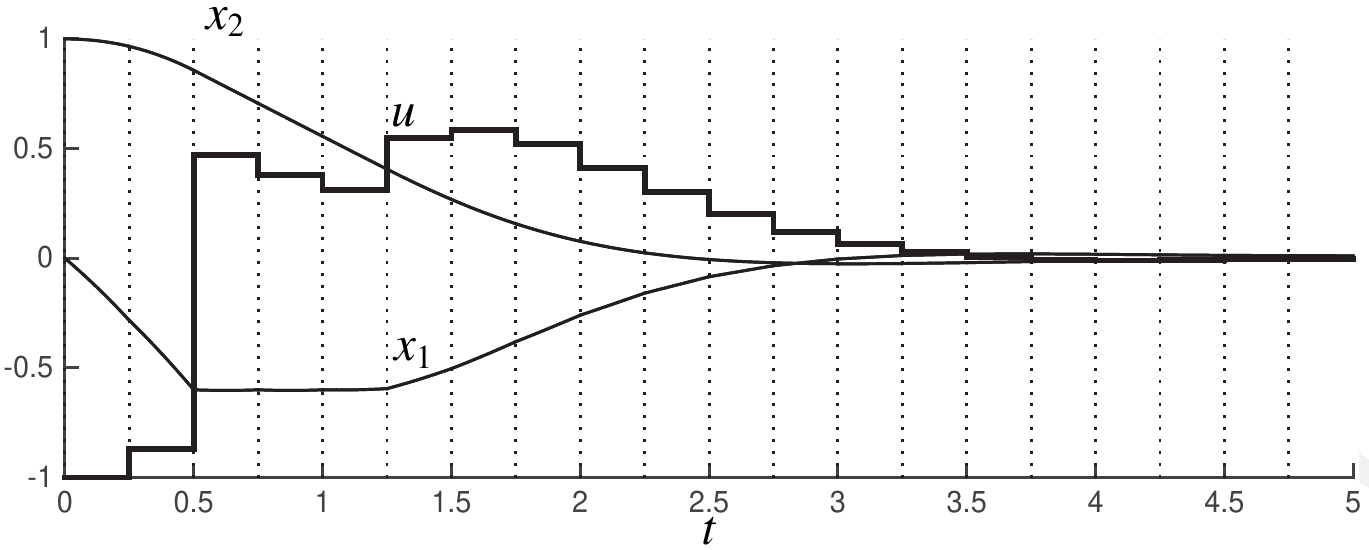
\includegraphics[width=0.8\textwidth]{direct_single_shooting}
\end{center}

  \begin{itemize}
  \item parametrize control function $u(t)$ into $N$ timesteps (polynomial of
    $n$-th grade, mostly $n=0$):
    \[u(t,q)=q_k,\quad t=[t_k,t_{k+1}],\quad q\in \mathbb{R}^N\]
  \item Forward simulate system dynamics
  \item Lower triangular jacobian of inequ. constraints
  \item Dense Hessian of Lagrange function
  \item Very good initial guess for $q$ required (difficult)\\
  \end{itemize}
  
\textbf{Direct multiple shooting:} corresponds to simultaneous approach\\
\begin{center}
  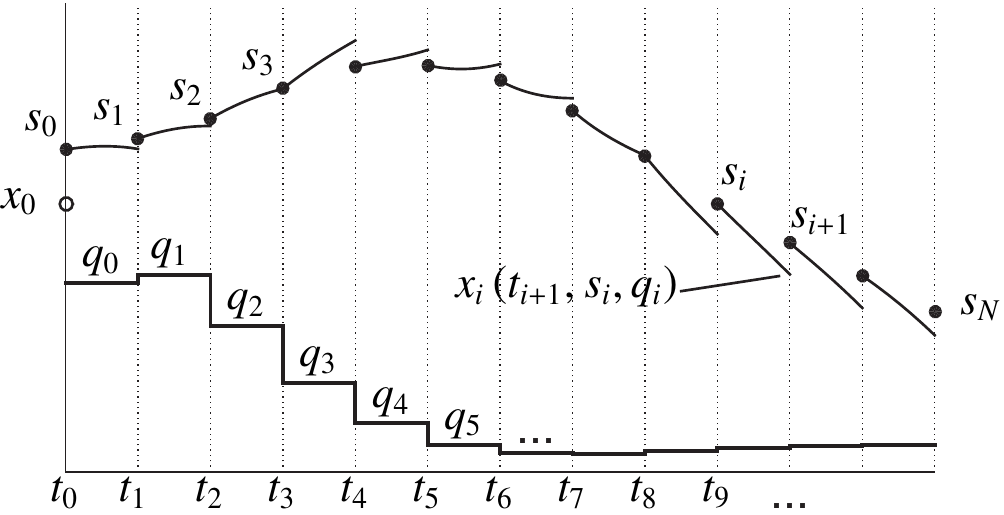
\includegraphics[width=0.8\textwidth,height=25mm]{direct_multiple_shooting}
\end{center}

  \begin{itemize}
  \item Same parametrisation as in single shooting
  \item Solve the ODE separately on each interval $[t_i,t_{i+1}]$:
    \begin{align*}
      \dot{x}_i(t, s_i, u_i) &= f(x_i(t,s_i,q_i),q_i) \\
      x_i(t_i,s_i,u_i) &= s_i
    \end{align*}
  \item Numerically integrate the cost over all intervals
  \item Additional continuity condition (piecing results together --- entails
    the system dynamics $f(x(t),u(t))$):
    \[s_{i+1}=x_i(t_{i+1},s_i,u_i)\]
  \item Eq. constraint ordering important (init. val.,
    continuity, path constr.) for sparsity structure
  \end{itemize}
  \textbf{Direct collocation:} Approximate states with polynomials (simultaneous
  as well)\\
  \begin{itemize}
  \item Parametrize $u(t)$ again (here: constant, i.e. $u(t)=q_k, t\in [t_k,t_{k+1}]$)
  \item Create polynomial fits $p_k(t, v_k)\in \mathbb{R}$ for each timestep $t_k$.
  \item Collocation equation (fitting system dynamics):
    \[c_k(v_k,s_k,q_k)=
      \left[
        \begin{array}{c}
          v_{k,0}-s_k \\
          \dot{p_k}(t_{k,1},v_k) - f(v_{k,1}, q_k) \\
          \vdots \\
          \dot{p_k}(t_{k,d},v_k) - f(v_{k,d}, q_k) \\
        \end{array}
      \right]=0,
      \quad
      \begin{array}{c}
        v_{k,i}\in \mathbb{R}^{n_x}\\
        i=0, \dots, d
      \end{array}
    \]
  \item Integrate $L$: $l_k(v_k,s_k,q_k) := \int^{t_{k+1}}_{t_k} L(x,u)\mathrm{d}t$
\item Collocation NLP:
\[
  \begin{array}{rrl}
    \min_{v,s,q}&\quad  E(s_N) + &\sum^{N-1}_{k=0} l_k(v_k,s_k,q_k) \\
    \mathrm{s.t.}&\quad s_0 - x_0 &= 0\quad \mathrm{(initial\ state)} \\
    &c_k(v_k,s_k,q_k) &= 0 \quad \mathrm{(collocation\ conditions)} \\ 
    &p_k(t_{k+1},v_k) - s_{k+1} &= 0\quad \mathrm{(continuity\ conditions)} \\
    &h(s_k,q_k)&\le 0\quad \mathrm{(path\ constraints)} \\
    & r(s_N) &\le 0\quad \mathrm{(terminal\ state)}
  \end{array}
\]
  \end{itemize}
\end{tcolorbox}
%%% Local Variables:
%%% mode: latex
%%% TeX-master: "../HelpSheet"
%%% TeX-engine: xetex
%%% End:

  \begin{tcolorbox}[colback=orange!5!white, %
  colframe=orange!75!black, %
  title=\textbf{Calculating Derivatives}]

\begin{center}
	\vspace{-0.2cm}
	\textbf{Methods to calculate a derivative}
	\vspace{-0.2cm}
\end{center}
\begin{enumerate}
	\item By hand (slow, error prone)
	\item Symbolic Differentiation (slow, long code, accurate to mach. prec.)
	\item Finite Differences (fast, inaccurate)
	\begin{center}
		\vspace{-0.1cm}
		$\nabla f(x)^Tp \approx \frac{f(x+tp)-f(x)}{t}$
		\vspace{-0.1cm}
	\end{center}
	Pitfalls: $t$ too small $\Rightarrow$ numerical cancellation errors,
	$t$ too big $\Rightarrow$ linearization errors. Rule of thumb: $t = \sqrt{\epsilon_{\text{mach}}}$ with $\epsilon_\text{mach}$ the machine precision.
	\item Imaginary trick in Matlab (fast, accurate to mach. pres). If $f$ is analytic and can be extended to complex numbers, then 
	\begin{center}
		\vspace{-0.1cm}
		$\nabla f(x)^Tp \approx \frac{\text{imag}(f(x+itp))}{t}$
		\vspace{-0.1cm}
	\end{center}
	This is closely related to forward AD.
	\item Algorithmic Differentiation (fast, accurate)
\end{enumerate}
\begin{center}
	\vspace{-0.1cm}
	\textbf{Algorithmic Differentiation Basics}
	\vspace{-0.2cm}
\end{center}
Each differentiable function $F:\mathbb{R}^n \to \mathbb{R}^{n_F}$ is composed of several ($m$) concatenated elementary operations $\Phi_i$ and a selection matrix $C$, i.e. 
\begin{center}
	\vspace{-0.1cm}
	$F(x) = C\cdot\Phi_{m}(\Phi_{m-1}(\dots\Phi_2(\Phi_1(x))\dots))$
	\vspace{-0.1cm}
\end{center}
The idea is to use the chain rule and differentiate each of the elementary operations separately $\Rightarrow$ Product of jacobians $J_i \in\mathbb{R}^{(n+i+1)\times (n+i)}$

\begin{center}
	\vspace{-0.1cm}
	$J_F = C \cdot J_{m} \cdot J_{m-1} \cdots J_2 \cdot J_1$
	\vspace{-0.0cm}
\end{center}

\begin{center}
	\vspace{-0.1cm}
	\textbf{Forward AD}
	\vspace{-0.2cm}
\end{center}
First define \grqq forward seed\grqq\ vector $p \in \mathbb{R}^n$ and then evaluate the directional derivative
\begin{center}
	\vspace{-0.2cm}
	$J_Fp = C \cdot (J_{m} \cdot (J_{m-1} \cdots (J_2 \cdot (J_1p)) \dots))$
	\vspace{-0.1cm}
\end{center}
One evaluation of forward AD gives us one \textbf{column} of the jacobian.

\textbf{Algorithm}
\begin{enumerate}
	\item Set $p$ to one of the unit vectors in $\mathbb{R}^n$
	\item Forward evaluation: Compute all intermediate values using the elementary operations
	\item Differentiation: Compute the dot quantities
	\item Output
\end{enumerate}

\textbf{Dot-Quantities:} $\dot{x}_i = \frac{\text{d}x_i}{\text{d}x}p$, \grqq how does the intermediate quantity depend on the input?\grqq

\textbf{Cost:} $\text{cost}(J_Fp) \leq 2 \cdot \text{cost}(F)$, $\text{cost}(J_F) \leq 2 \cdot n \cdot \text{cost}(F)$

\textbf{Advantages:} Low storage requirements, step 2 and 3 parallelizable

\textbf{Useful for:} Functions with few inputs or equally many inputs as outputs

\begin{center}
	\vspace{-0.1cm}
	\textbf{Backward AD}
	\vspace{-0.2cm}
\end{center}
First define the \grqq backward seed\grqq\ vector $\lambda \in \mathbb{R}^n$ and then evaluate the (transposed) directional derivative
\begin{center}
	\vspace{-0.1cm}
	$J_F^T\lambda = J_1^T \cdot (J_2^T \cdots (J_{m-1}^T \cdot (C^T\lambda))\dots))$
	\vspace{-0.1cm}
\end{center}
One evaluation of backward AD gives us one \textbf{row} of the jacobian.

\textbf{Algorithm:}
\begin{enumerate}
	\item Set $\lambda$ to one of the unit vectors in $\mathbb{R}^{n_F}$, set bar quantities to zero
	\item Forward evaluation: Compute intermediate variables using elementary operations
	\item Backward sweep: Go through each elementary operation in reverse and update the bar quantities using the update rule below
	\item Output 
\end{enumerate}
\textbf{Bar-quantity:} $\bar{x}_i = \lambda^T\frac{\text{d}F}{\text{d}x_i}$, \grqq How does the output $\lambda^TF(x)$ depend on the intermediate variable $x_i$?\grqq

\textbf{Cost:} $\text{cost}(\lambda^TJ_F) \leq 3 \cdot \text{cost}(F)$, 
$\text{cost}(J_F) \leq 3 \cdot n_F \cdot \text{cost}(F)$

\textbf{Disadvantage:} High storage requirements

\textbf{Useful for:} Functions with fewer outputs than inputs

\textbf{Update rule:} Regard operation $x_{n+i+1} = \Phi_i(x_j,x_k)$, then
\begin{center}
	\vspace{-0.1cm}
	$\bar{x}_j = \bar{x}_j + \frac{\partial \Phi_i}{\partial x_j} \cdot \bar{x}_{n+i+1}$ and
	$\bar{x}_k = \bar{x}_k + \frac{\partial \Phi_i}{\partial x_k} \cdot \bar{x}_{n+i+1}$
\end{center}

\begin{center}
	\vspace{-0.1cm}
	\textbf{Efficient Hessian Computation}
	\vspace{-0.2cm}
\end{center}
Regard a Lagrangian function (or any objective) $f:\mathbb{R}^n \to \mathbb{R}$ of which we want to compute the hessian $\nabla^2 f(x)$. With finite differences we need at least $n(n+1)/2$ function evaluations. Better: First use backward AD to compute jacobian, then use forward AD to compute hessian. Total cost: $\text{cost}(\nabla^2 f) \leq 6 \cdot n \cdot \text{cost}(f)$
\end{tcolorbox}

%%% Local Variables:
%%% mode: latex
%%% TeX-master: "../HelpSheet"
%%% End:
  \begin{tcolorbox}[colback=violet!5!white, %
  colframe=violet!75!black, %
  title=\textbf{Parametric Nonlinear Optimization}]
  \textbf{General problem formulation of parametric programming:}
  \begin{align*}
    w^*(p)=\argmin_w \quad&f(w,p) \\
    \text{s.t.}\quad & g(w,p)=0 \\
    & h(w,p) \le 0
  \end{align*}
  With $y:=(w,\lambda,\mu)$, the KKT conditions can be re-stated as:
  \begin{align*}
    R_\text{A}(y,p)=
    \left[
    \begin{array}{c}
      \nabla_w \mathcal{L}(y,p) \\
      g(w,p) \\
      h_A(w,p) \\
      \mu_{\bar{\text{A}}}
    \end{array}
    \right] = 0,\quad h_{\bar{\text{A}}}(w,p) < 0,\quad \mu_\text{A} > 0
  \end{align*}
  For any neighbourhood of a given $\bar{p}$ and $w^*(\bar{p})$:
  ($y^*_\text{A}:=(w^*,\lambda^*, \mu^*_{\text{A}})$)
  \begin{align*}
    &\left.\underbrace{\left[\begin{array}{ccc}
            \nabla^2_{ww}\mathcal{L}&\nabla_w g&\nabla_w h \\
            \nabla_w g^\top& 0 & 0 \\
            \nabla_w h^\top& 0 & 0
          \end{array}\right]}_{\text{KKT-Matrix}}
                                 \frac{\partial y_\text{A}^*}{\partial p} +
                                 \frac{\partial}{\partial p}
                                 \left[
                                 \begin{array}{c}
                                   \nabla_w \mathcal{L} \\
                                   g \\
                                   h_\text{A}
                                 \end{array}
    \right]\right|_{p=\bar{p}} = 0,\\
    &\frac{\partial\mu^*_{\bar{\text{A}}}}{\partial p} = 0
  \end{align*}
  Predictor-Corrector-Algorithm (for inequ. constr. free problems):
  \begin{itemize}
  \item Start with initial values for $k_0, z_0, p_0$
  \item for $k=0,1,\dots$:
    \begin{itemize}
    \item Get new estimate $p_{k+1}$
    \item Generate new approx. solution $y_{k+1}$
    \end{itemize}

  \end{itemize}
  \begin{align*}
    y_{k+1}=y_k - 
    &\left(
    \frac{\partial R}{\partial y}(y_k, p_k)
    \right)^{-1} \\
    & \cdot
    \left(
      \underbrace{R(y_k, p_k)}_{\text{Correction-step (Newton)}} +
      \underbrace{\frac{\partial R}{\partial p}(y_k, p_k)(p_{k+1} - p_k)}_{\text{Tangential predictor}}
    \right)
  \end{align*}
  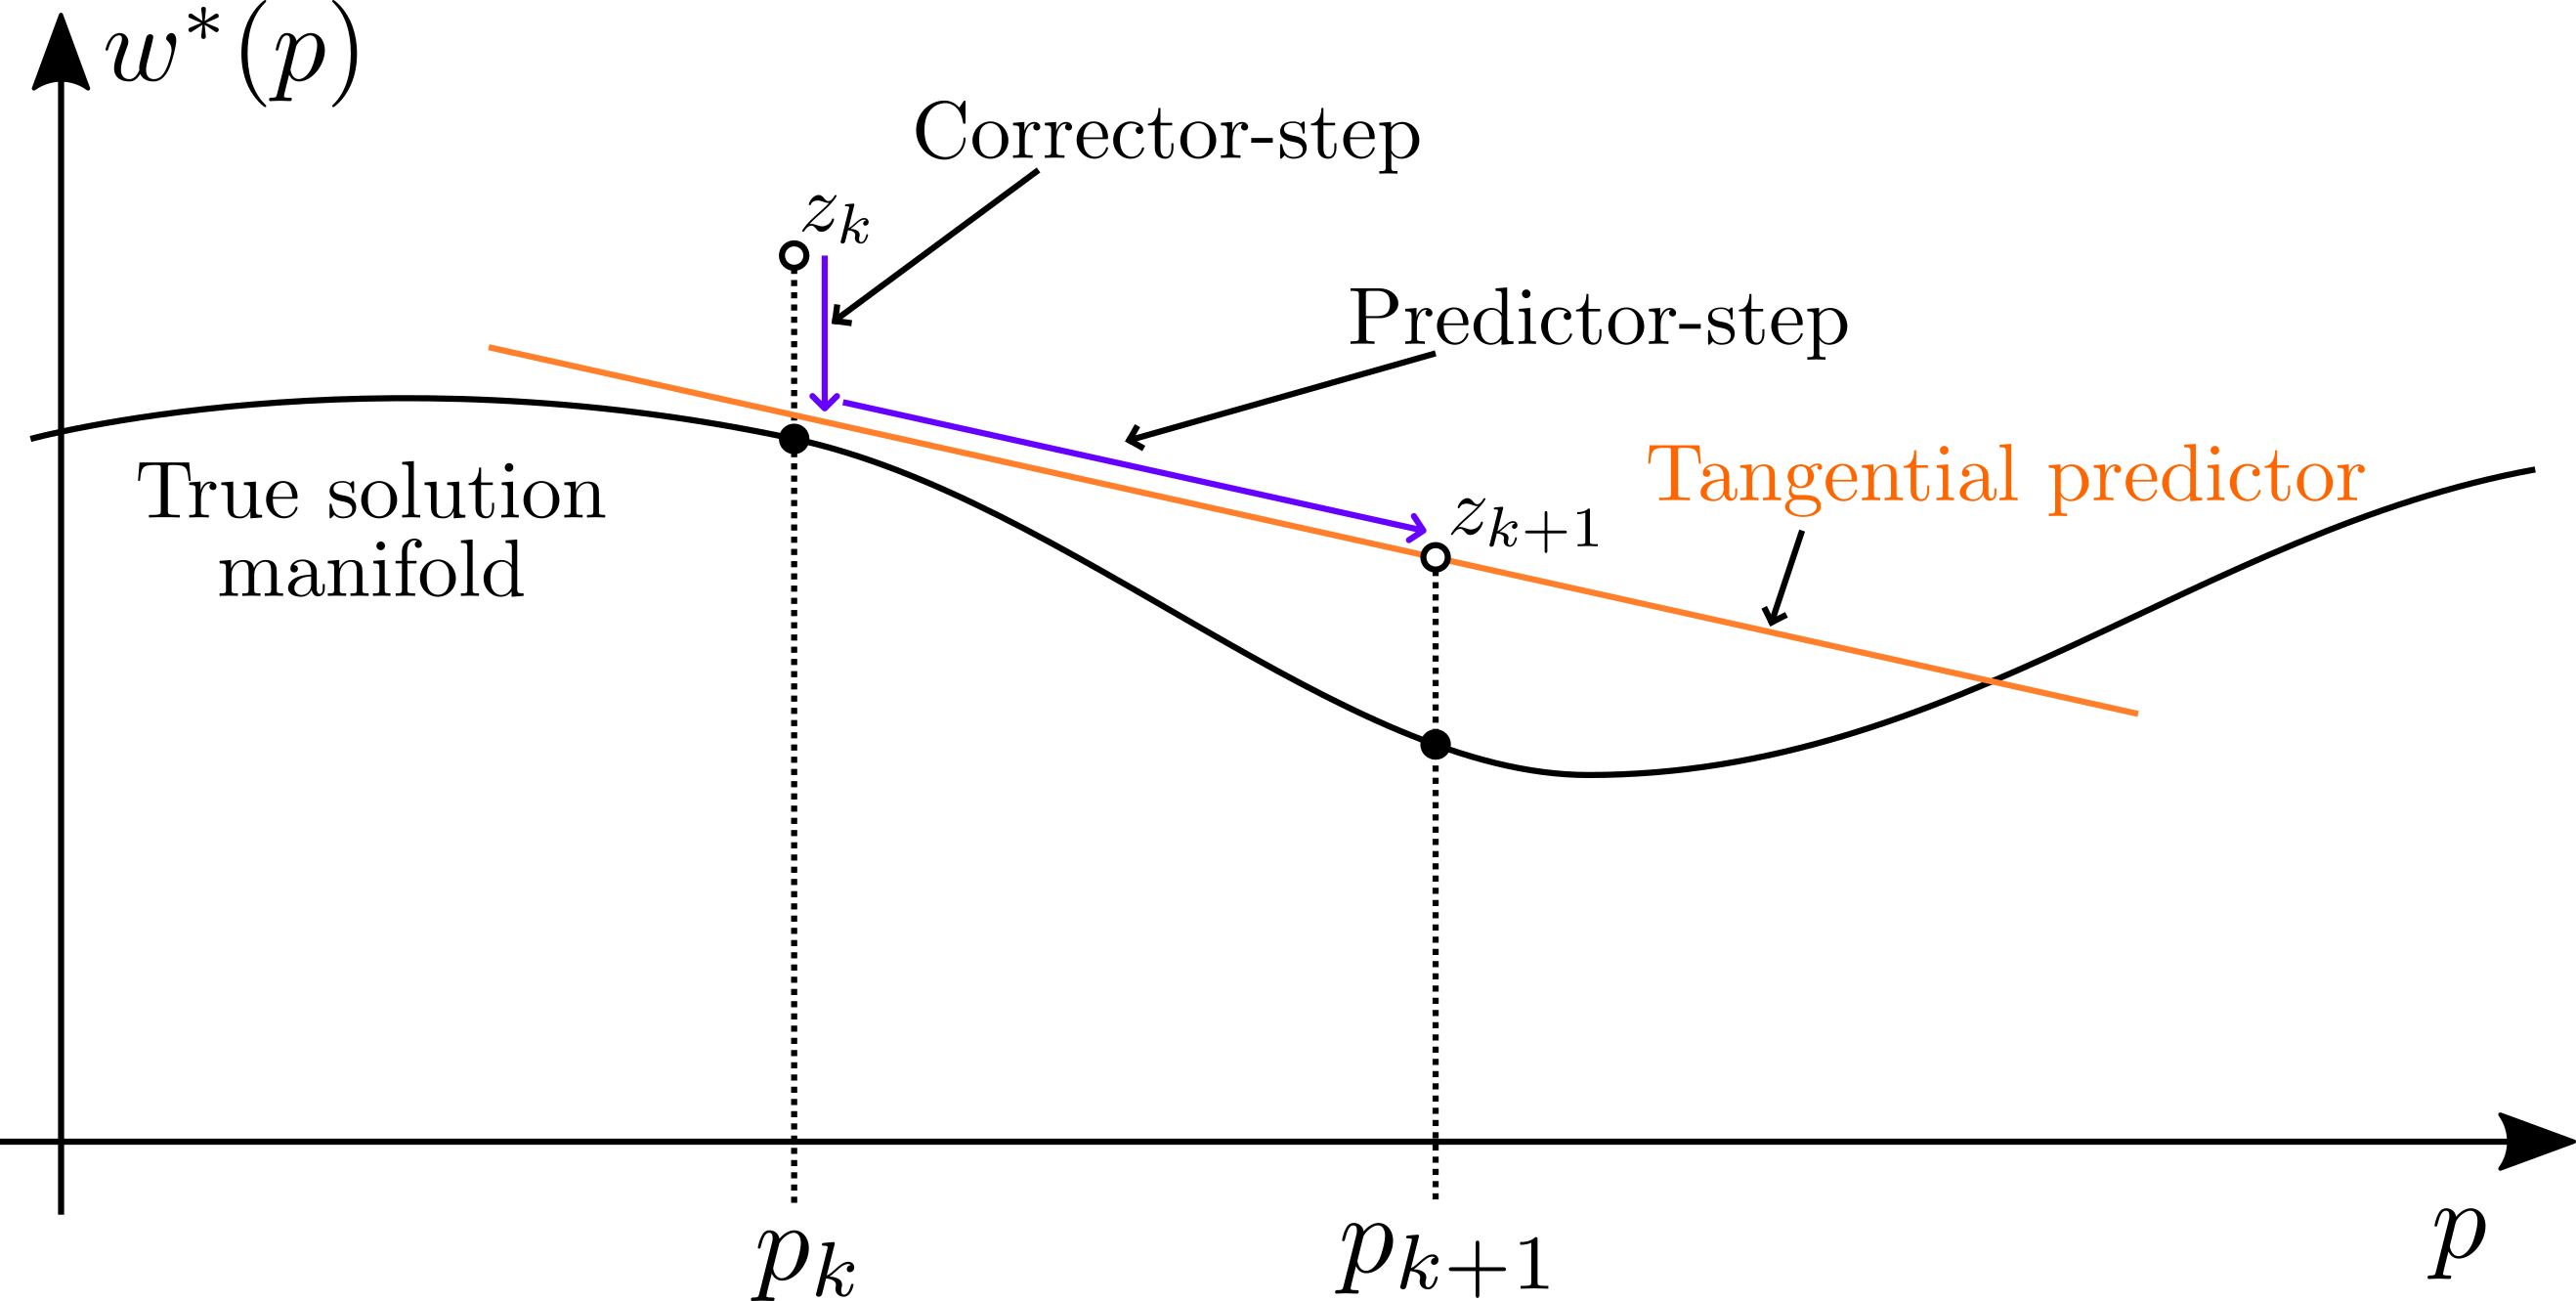
\includegraphics[width=0.8\textwidth]{pred_correct_alg}

  
\end{tcolorbox}

%%% Local Variables:
%%% coding: utf-8
%%% mode: latex
%%% TeX-engine: xetex
%%% TeX-master: "../HelpSheet"
%%% End:
  \begin{tcolorbox}[colback=green!5!white,
  colframe=green!75!black,
  title=\textbf{Numerical integration/simulation}]
  \textbf{Explicit Runge-Kutta:} use $m$ evaluations each timestep $s_k$ with
  \[\lim_{N\rightarrow\infty}s_k=x(t_k)\]
  Intermediate time points:
  \[t_{k,i}:= t_k + c_i\Delta t,\quad c_i\in [0,1]\]
  \begin{align*}
    s_{k, 1} &:= s_k \\
    s_{k, 2} &:= s_k + \Delta t\cdot a_{21}\cdot f(s_{k,1}, t_{k,1}) \\
    s_{k, 3} &:= s_k + \Delta t(a_{31}\cdot f(s_{k,1}, t_{k,1}) + a_{32}\cdot f(s_{k,2}, t_{k,2}))\\
    s_{k, i} &:= s_k + \Delta t\sum^{i-1}_{j=1}a_{ij}\cdot f(s_{k,j}, t_{k,j}) \\
    s_{k+1} &:= s_k + \Delta t \sum^m_{j=1}b_j\cdot f(s_{k,j}, t_{k,j})
  \end{align*}
  With the \emph{Butcher-Tableau:}
  \begin{equation*}
    \resizebox{!}{11mm}{$
      \begin{array}{c|cccc}
        \multicolumn{5}{c}{\mathrm{{\Large General\ case}}}\\
      c_1&&&& \\
      c_2&a_{21}&&& \\
      c_3&a_{31}&a_{32}&& \\
      \vdots & \ddots & \ddots&& \\
      c_m & a_{m1} & \dots & a_{m,m-1} & \\ \hline
      & b_1 & b_2 & \dots & b_m
    \end{array}
    $}
  \hspace{15pt}
  \begin{array}{c|cccc}
    \multicolumn{5}{c}{\mathrm{RK4}}\\
      0&&&& \\
      0.5&0.5&&& \\
      0.5&0&0.5&& \\
      1 & 0 & 0 & 0.5 & \\ \hline
      & \frac{1}{6} & \frac{1}{3} & \frac{1}{3} & \frac{1}{6}
    \end{array}
  \end{equation*}\\

  \textbf{Implicit RK:}
  \begin{itemize}
  \item Square Butcher-Tableau
  \item Nonlinear system of equations, solved with Newton method\\
  \end{itemize}

  \textbf{Orthogonal collocation:} approximate $x(t)$ on interval
  $t\in[t_k,t_{k+1}]$ with polynomial $p_t,v_k\in \mathbb{R}^n$
  \begin{itemize}
  \item Built from Lagrange polynomials on set of collocation times
    $t_{k,0},\dots,t_{k,d}$:
    \begin{align*}
      p_k(t,v_k)&=\sum^d_{i=0}v_{k,i}l_{k,i}(t),\\
      l_{k,i}(t)&=\prod^d_{j=0,j\ne i}\frac{t-t_{k,i}}{t_{k,i}-t_{k,j}}\in\mathbb{R} \\
      \Rightarrow l_{k,i}(t_{k,j})&=
                                    \left\{ 
                                    \begin{array}{l}
                                      1\ \mathrm{if}\ i=j \\
                                      0\ \mathrm{if}\ i\ne j
                                    \end{array}
      \right.
    \end{align*}
  \item To get proper approximations, solve the \emph{collocation equations}:
    \begin{align*}
      c_k(v_k,t_{k,i},s_k)=
      \left[
      \begin{array}{c}
        v_{k,0}-s_k \\
        \dot{p}_k(t_{k,1},v_k) - f(v_{k,1},t_{k,i}) \\
        \dots \\
        \dot{p}_k(t_{k,d},v_k)-f(v_{k,d},t_{k,i})
      \end{array}
      \right] = 0
    \end{align*}
  \item Collocation times $c_i\in [0,1]$: zeros of orthogonal Legendre
    polynomials on $[t_k,t_{k+1}]$
    \begin{align*}
      \begin{array}{cc}
        d & c_i \\ \hline
        1 & 0.5 \\
        2 & 0.5 \pm \sqrt{\frac{1}{3}} \\
        3 & 0.5, 0.5 \pm \sqrt{\frac{3}{5}} \\
        4 & 0.5 + \pm\sqrt{\frac{3}{7} \pm \frac{1}{7}\sqrt{\frac{24}{5}}}\\
      \end{array}
    \end{align*}
  \end{itemize}
\end{tcolorbox}
%%% Local Variables:
%%% coding: utf-8
%%% mode: latex
%%% TeX-engine: xetex
%%% TeX-master: "../HelpSheet"
%%% End:

  
\begin{tcolorbox}[colback=lime!5!white,%
  colframe=lime!75!black,%
  title=\textbf{Sequential and Simultaneous approach}]
  \textbf{Basic problem formulation}
  \begin{align*}
    \begin{array}{|rl|}\hline
    \min_w &F(w) \\
    \mathrm{s.t.}\quad & G(w) \\ \hline
    \end{array}

  \end{align*}
  \textbf{KKT for simultaneous approach}
\end{tcolorbox}
%%% Local Variables:
%%% mode: latex
%%% TeX-master: "../HelpSheet"
%%% TeX-engine: xetex
%%% End:

  \begin{tcolorbox}[colback=blue!5!white, %
  colframe=blue!75!black, %
  title=\textbf{Predictor-Corrector Path-following for RT-OC and NMPC}]
  $p=x_0$ is the parameter on which parameter optimization hinges.
  ``Generalized tangential predictor'' can jump over active set changes (that's
  where the trajectory manifold has kinks).
  \begin{itemize}
  \item \textbf{GMRES method of Ohtsuka}
    \begin{itemize}
    \item Sequential (single-shooting)
    \item IP method, with fixed $\tau>0$
    \item Exact Hessian\\
    \end{itemize}
    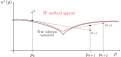
\includegraphics[width=0.8\textwidth]{ohtsuka}
  \item \textbf{Advanced step controller}
    \begin{itemize}
    \item Solve NLP for a predicted parameter $\bar{p}_{k+1}$
    \item get $\nabla_p w^*(p)$ from KKT matrix
    \item when real parameter $p_{k+1}$ arrives:
      \begin{align*}
        y^*_{k+1} = \bar{y}_{k+1}(\bar{p}_{k+1})+\nabla_pw^*(\bar{p}_{k+1})(p_{k+1} - \bar{p}_{k+1})
      \end{align*}
    \end{itemize}
    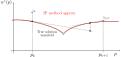
\includegraphics[width=0.8\textwidth]{advanced_step}
  \item \textbf{Real-Time Iteration Scheme}
    \begin{itemize}
    \item Preprocess SQP with inputs $y_k, p_{k+1}$:
      \begin{align*}
        \min_w \quad&f(w) \\ \mathrm{s.t.}\quad& g(w) + M\cdot p = 0,& M:=[\mathbb{I}^{n_x}, 0, \dots] \\ & h(w) \le 0
      \end{align*}
      \begin{align*}
        \Rightarrow \min_w \quad & \nabla_w f(w)^T\cdot (w-w_k) + 0.5 \nabla^2_w \mathcal{L}(y)\cdot(w-w_k) \\
        \mathrm{s.t.}\quad& g(w) + \nabla_w g(w_k)\cdot(w-w_k) - Mp_{k+1} = 0 \\
        & h(w) + \nabla_w h(w_k)\cdot(w-w_k)\le 0
      \end{align*}
    \item Just perform \emph{one} linearization and one QP solution
    \item Often used: Gauss-Newton-Hessian
    \item Works well when the active set changes faster than the linearized
      system matrices
    \item Warm-start the state
    \end{itemize}

  \end{itemize}
\end{tcolorbox}

%%% Local Variables:
%%% coding: utf-8
%%% mode: latex
%%% TeX-engine: xetex
%%% TeX-master: "../HelpSheet"
%%% End:
  
\end{multicols*}

% TODO: Discretization methods (e.g. RK4)
% TODO: Collocation

\end{document}

%%% Local Variables:
%%% coding: utf-8
%%% mode: latex
%%% TeX-engine: xetex
%%% TeX-master: t
%%% End:
